\chapter{L-Système}

\section{Principe et fonctionnement}

\subsection{Qu'est-ce que le L-Système ?}
Le L-Système \footnote{Le système de Lindebmayer}, inventé en 1968 par un biologiste hongrois du nom de Aristid Lindenmayer, est un système de réécriture \footnote{Modèle de calcul transformant des objets syntaxiques comme des mots, des termes ou encore des graphes en appliquant des règles données.} utilisé pour la modélisation de processus de développement et de prolifération de bactéries ou de plantes.

\subsection{Comment fonctionne-t-il ?}
Ce système de réécriture fonctionne par le biais de plusieurs spécificités :
\begin{itemize}
    \item Un alphabet : celui-ci est l'ensemble des variables et des constantes utilisées.
    \item Un axiome : il représente le point de départ, l'état initial du système.
    \item Des règles de réécriture : elles définissent les règles de développement du L-Système en utilisant l'alphabet donné dans le but de créer un mot.
\end{itemize}
En additionnant tous ces aspects, nous obtenons alors notre L-Système, commençant par l'axiome étant la base, puis, créant au fur et à mesure un mot grâce aux règles données (Dans la limite du nombre d'itérations imposés \footnote{Le nombre d'itérations ou nombre de générations correspond au nombre de réécritures de l'axiome pour obtenir le mot final}), tout ceci étant possible grâce à l'alphabet qui les composes.
Ce mot passera ensuite par un moteur graphique dans le but d'être modélisé.

\section{Notre L-Système}

\subsection{Alphabet}
\label{sec:Alphabet}
Notre alphabet est composés de plusieurs règles et constantes :\\
\begin{itemize}
    \item X permet de dessiner une branche et Y de ne rien dessiner, ils permettent avec certaines règles de contrôler l'évolution de notre L-Système.
    \item Il est possible de modifier l'angle d'une branche en utilisant par exemple les +, -, -35, +64y, qui donnera respectivement une orientation de 25° et -25° sur l'axe de rotation x, une rotation de -35° sur l'axe X et une orientation de 64° sur l'axe de rotation y ; il n'est pas possible de modifier l'orientation de l'axe de rotation Z.
\result{Exemple : +XYX appliquera une rotation de 25° a X et aucune à Y et au 2ème X}
\item Enfin il est possible d'utiliser les crochets [] pour contrôler l'évolution et obtenir des branches à vos arbres. Ces crochets vont conserver l'état, c’est-à-dire qu'une rotation appliquée aux crochets s'appliquera a tous les éléments étant à l'intérieur des crochets. Il est possible d'imbriquer des crochets.\\
\result{Exemple : +[XYX] appliquera une rotation de 25° à XYX.}
\end{itemize}

\subsection{Axiome, règles de réécritures et nombre d'itérations}
Pour l'axiome, les règles de réécritures et le nombre d'itérations, ils seront définis par l'utilisateur dans les zones de textes de l'interface prévus a cet effet. 
Un bouton "Aide" est présent sur cette même interface aidant à comprendre et mettre en place le L-Système.

\begin{figure}[h!]
    \centering
    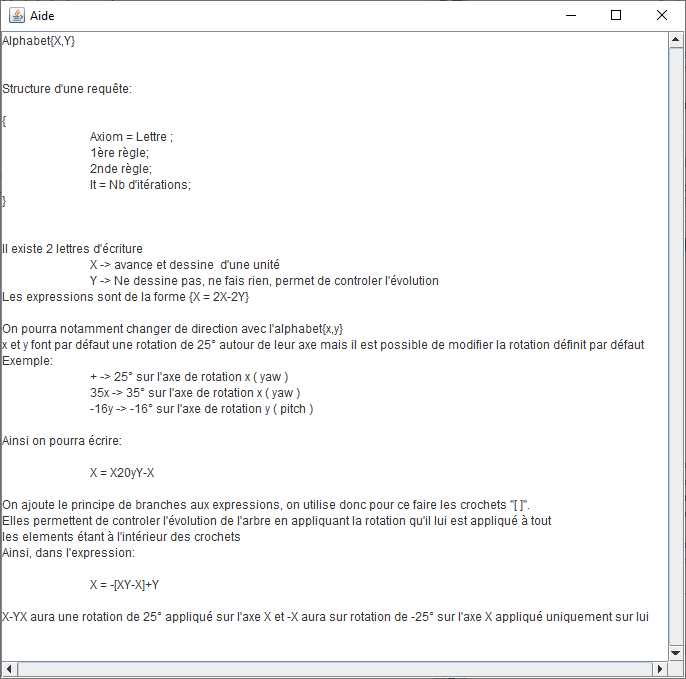
\includegraphics[width=0.8\linewidth]{pics/aideGUI.png}
    \caption{Fenêtre d'aide}
    \label{fig:help_frame}
\end{figure}
